\begin{frame}{Simple Photoemission from a Metal}
  \begin{center}
  \begin{tikzpicture}[every node/.style={transform shape}]
    \node (electron) [circle,fill=pink,draw,label=above left:{\Large e$^{-}$}] {};
    \fill [blue!50] 
      ($(electron) + (-2cm,-3cm)$) node [left,black] {\Large $\varepsilon_{\scriptscriptstyle F} $}
      -- ++(+2cm,0) node (surface) {}
      -- ++(0,-2cm) node (sub-surface) {}
      -- ++(-2cm,0);
    
    \draw [gray,line width=2mm,->,>=latex']
      (surface.center) 
      -- (electron) node [midway] (photon) {};
    
    \draw [line width=1.5mm,<-,>=latex,decorate,blue,decoration={snake,pre=lineto,pre length=7mm}]
      (photon)
      -- ++(-2cm,0) node [midway,above=3mm,black] {\large $ \hbar \omega $};
      
    \draw [gray,line width=0.5mm] 
      (surface) ++(1cm,0) -- ++(3cm,0) node [pos=0.3] (x-phi) {};
  
    \draw [line width=0.7mm,dashed]
      (surface.center) to [out=80,in=180] ($(electron -| x-phi) + (0,5mm)$) -- ++(2cm,0) node [label=above right:{$ E_{DC}=0 $}] (upper-no-field) {};
    \draw [line width=0.7mm]
      (sub-surface.center) -- (surface.center) to [out=80,in=160] ($(electron -| x-phi) - (0,4mm)$) node (upper) {} -- ++(-20:2.2cm);
  
    \draw [line width=1mm,->,>=latex,pink] 
      (electron) -- ++(5cm,0) 
        node (exit) {}
        node [right,black] {$\Delta p_{\smallT} = \sqrt{\frac{m (\hbar \omega - \Phi_{eff})}{3}}$};
    \node [below=of exit,shape=single arrow,minimum height=1cm,draw,fill=red,label={[yshift=-5mm]below:{$ E_{DC} $}},rotate=180] {};
    
    \draw [<->,>=latex] (x-phi) -- (upper) node [pos=0.4,right] {\large $ \Phi_{eff} < \Phi $};
    \draw [<->,>=latex] (upper-no-field) -- (upper-no-field |- surface.north);

    \node<2-> [red] at (4cm,-4cm) {$\eta_{PE} = A (1-R) (\hbar \omega - \Phi_{eff})^2$};
  \end{tikzpicture}
  \end{center}
\end{frame}

\begin{frame}{Driving a Plasmon (Back-Illuminated)}
  \begin{columns}
  \begin{column}{0.54\linewidth}
    \begin{center}
    \begin{tikzpicture}
      \filldraw [fill=gray!10]
      (0,0)
      node [below left] {Glass}
      rectangle (-2,-5)
      ;
      \filldraw
        [fill=orange]
        (0,0) 
        node [name=photocathode1,above right]{Au Film ($\varepsilon$)}
        -- ++(0.2,0)
        -- ++(0,-5)
        node [name=source,midway] {} 
        -- ++(-0.2,0)
        -- (0,0)
        node [name=laser,midway] {}
        -- cycle
      ;
      \draw
        [-latex,ultra thick,green] 
        ($(laser) + (-135:3.5)$) 
        -- (laser.west)
        node [left=0.3,name=laser label,pos=0.8,black,fill=white] {Laser ($\lambda$)}
      ;
      \fill
        [blue!30]
        (source.center)
        -- ++(3,2mm)
        -- ++(0,-4mm)
        -- cycle
      ;
      \draw
        [-latex,ultra thick,blue]
        (source.center)
        -- ++(3,2mm)
      ;
      \draw
        [-latex,ultra thick,blue]
        (source.center)
        -- ++(3,-2mm)
        node [name=electron label,pos=0.5,black,below=0.2,align=center]{Photoemitted\\Electrons}
      ;
      \draw
        [dashed]
        (source)
        -- ++(3.3,0)
      ;
      \draw 
        ($(laser) + (0,-1)$) 
        arc (-90:-135:1)
        node [below=0.3] {$\theta$}
      ;
    \end{tikzpicture}
    \end{center}
  \end{column}
  \begin{column}{0.44\linewidth}
    \begin{figure}
      \centering
      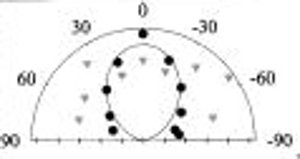
\includegraphics[scale=0.8]{plasmon_reduction_angle}
      \caption{The measured angular distribution of photoelectrons
in the plane of incidence (dots) and perpendicular to that (triangles), as
well as a fit to a $\cos^2\theta$ distribution.\footcite{zawadzka_evanescent}}
    \end{figure}
  \end{column}
  \end{columns}
\end{frame}

\begin{frame}{Driving a Plasmon (Front-Illuminated)}
  \begin{columns}
    \begin{column}{0.49\linewidth}
  \begin{center}
  \begin{tikzpicture}
    \filldraw
      [fill=orange]
      (0,0) 
      node [name=photocathode1,below right]{Au}
      node [below=1mm of photocathode1] {$\varepsilon$}
      -- ++(1,0)
      decorate [decoration=snake,segment length=5mm]{ 
        -- ++(0,-5)
        node [name=source,midway] {} 
      } 
      -- ++(-1,0)
      -- cycle
    ;
    \draw [|-|]
      ($(source) + (-4mm,-14mm)$)
      -- ++(0,-5mm)
      node [midway,left] {$a$}
    ;
    \begin{pgfonlayer}{background}
      \foreach \x in {8.5mm,3.5mm,-1.5mm,-6.5mm} {
        \fill<2->
          [fill=red]
          ($(source) + (0,\x)$) 
          ellipse (6mm and 2.5mm)
        ;
        \fill<2->
          [fill=red!50]
          ($(source) + (0,\x)$)
          ellipse (3mm and 1.5mm)
        ;
      }
    \end{pgfonlayer}
    \draw
      [-latex,ultra thick,green] 
      ($(source) + (45:3.5)$) 
      -- (source.east)
      node [name=laser label,pos=0.3,black,fill=white] {Laser ($\lambda$)}
    ;
    \fill<3->
      [blue!30]
      (source.east)
      -- ++(3,2mm)
      -- ++(0,-4mm)
      -- cycle
    ;
    \draw<3->
      [-latex,ultra thick,blue]
      (source.east)
      -- ++(3,2mm)
    ;
    \draw<3->
      [-latex,ultra thick,blue]
      (source.east)
      -- ++(3,-2mm)
      node [name=electron label,pos=0.8,black,above=0.5,align=center]{Photoemitted\\Electrons}
    ;
    \draw
      [dashed]
      (source)
      -- ++(4,0)
    ;
    \draw 
      ($(source) + (1,0)$) 
      arc (0:41:1)
      node [right=0.3] {$\theta$}
    ;
    \node<2-> [anchor=west,align=center] at ($(source) + (0.3,-1.2)$) {Plasmon\\Oscillation};
  \end{tikzpicture}
  \end{center}
    \end{column}
    \begin{column}{0.49\linewidth}
      To drive a surface plasmon by front-illumination align so that:
      \begin{align*}
        k_{SP} =& k_{laser}^{\parallel} + k_{G}\\
        \sin(\theta) =& \sqrt{ \frac{\varepsilon}{1+\varepsilon} } - \frac{\lambda}{a}
      \end{align*}
      where $\varepsilon$ is the metal's dielectric constant
      \begin{block}<4->{Why Gold?}
        Surface plasmon frequency is near 2nd harmonic (green) of our Yb:KGW laser
      \end{block}
    \end{column}
  \end{columns}
\end{frame}

\begin{frame}{First Attempt (Gold on Glass)}
  \begin{columns}
    \begin{column}{0.49\linewidth}
      First attempt:
      \begin{itemize}
        \item Commercial optical grating
        \item Gold on glass substrate
        \item 750 lines per mm
      \end{itemize}
      \visible<2->{
        \begin{block}{Result}
          Insufficient heat conduction though glass substrate
        \end{block}
      }
    \end{column}
    \begin{column}{0.49\linewidth}
      \begin{figure}
        \centering
        \visible<2->{
          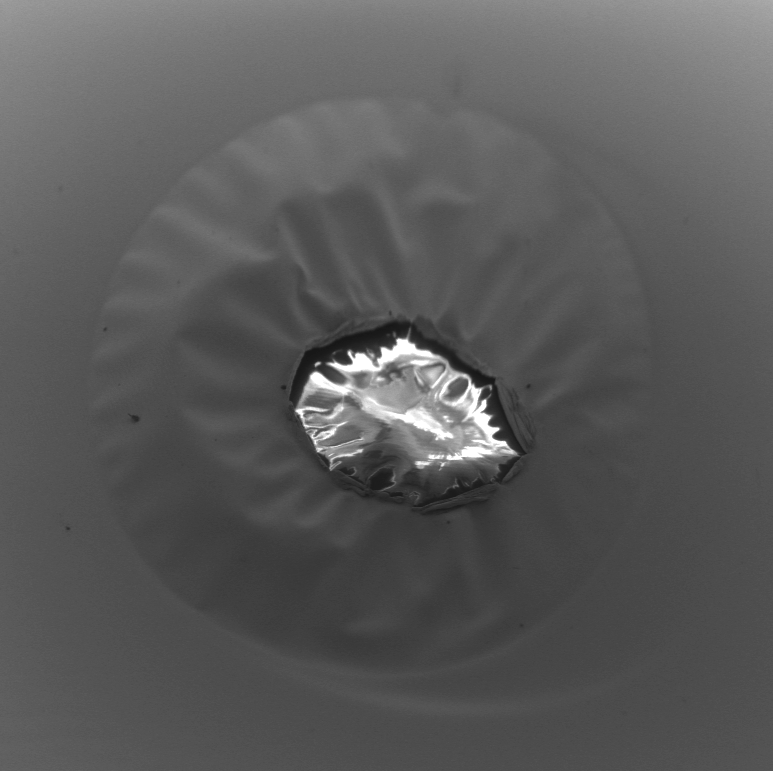
\includegraphics[width=0.8\linewidth]{Damage}
        }
      \end{figure}
    \end{column}
  \end{columns}
\end{frame}

\begin{frame}{Second attempt (Gold on FIB milled silicon)}
  To avoid heat problems:
  \begin{itemize}
    \item Silicon substrate
    \begin{itemize}
      \item Focused Ion Beam (FIB) milled at Argonne Nat'l Lab (ANL)
      \item Near sinusoidal shape
      \item $\sim 1 \mu$m periodicity
      \item Several ($\sim10$) 100$\mu$m x 100$\mu$m patches
      \item Several hours of milling
    \end{itemize}
    \item Gold coated at UIC Nano Core Facility (NCF)
    \begin{itemize}
      \item 300 nm thickness
      \item Chromium binding layer
    \end{itemize}
  \end{itemize}
  
\end{frame}

\begin{frame}{Sinusoidal Nanopatterned Photocathode}
  \begin{tikzpicture}
    \begin{pgfonlayer}{below-main}
      \node[name=low,label=below:Low Mag]{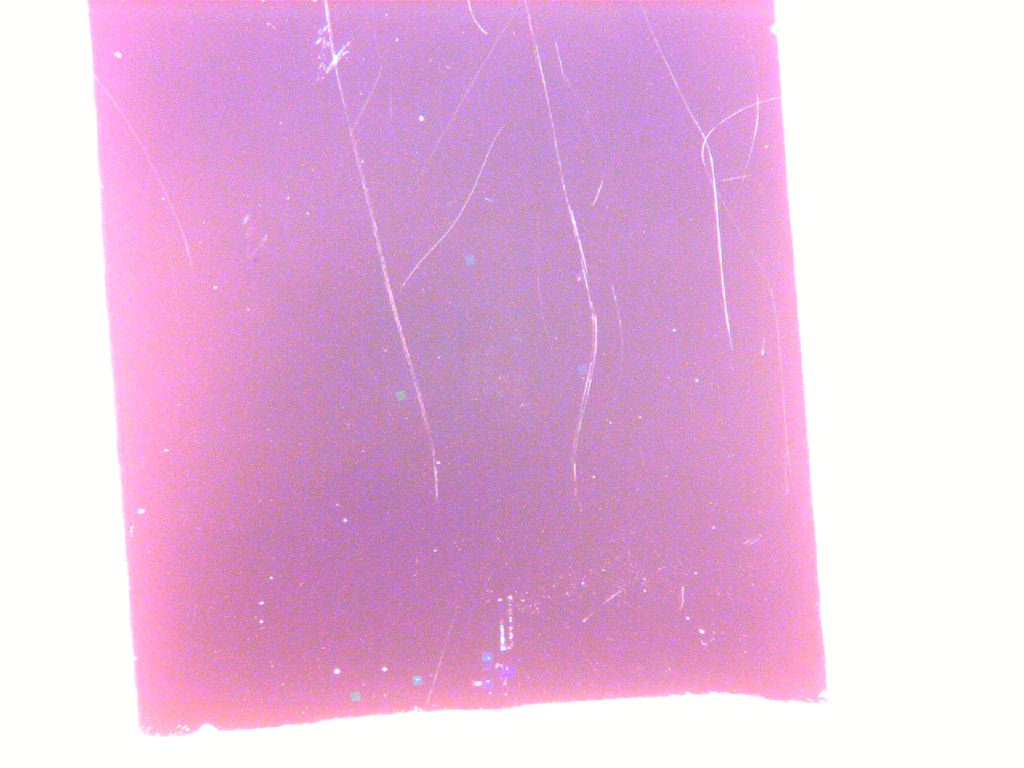
\includegraphics[width=2in]{FIB-low}};
    \end{pgfonlayer}
    \draw<2->
      (-7mm,8mm) node [name=low-top-left] {}
      -- ++(12mm,0) node [name=low-top-right] {}
      -- ++(0,-10mm) node [name= low-bottom-right] {}
      -- ++(-12mm,0) node [name= low-bottom-left] {}
      -- cycle
    ;
    \visible<3->{
      \node [
        inner sep=0,
        right=8mm of low.center,
        yshift=2.3cm,
        name=medium,
        label=above:Medium Mag
      ] {
        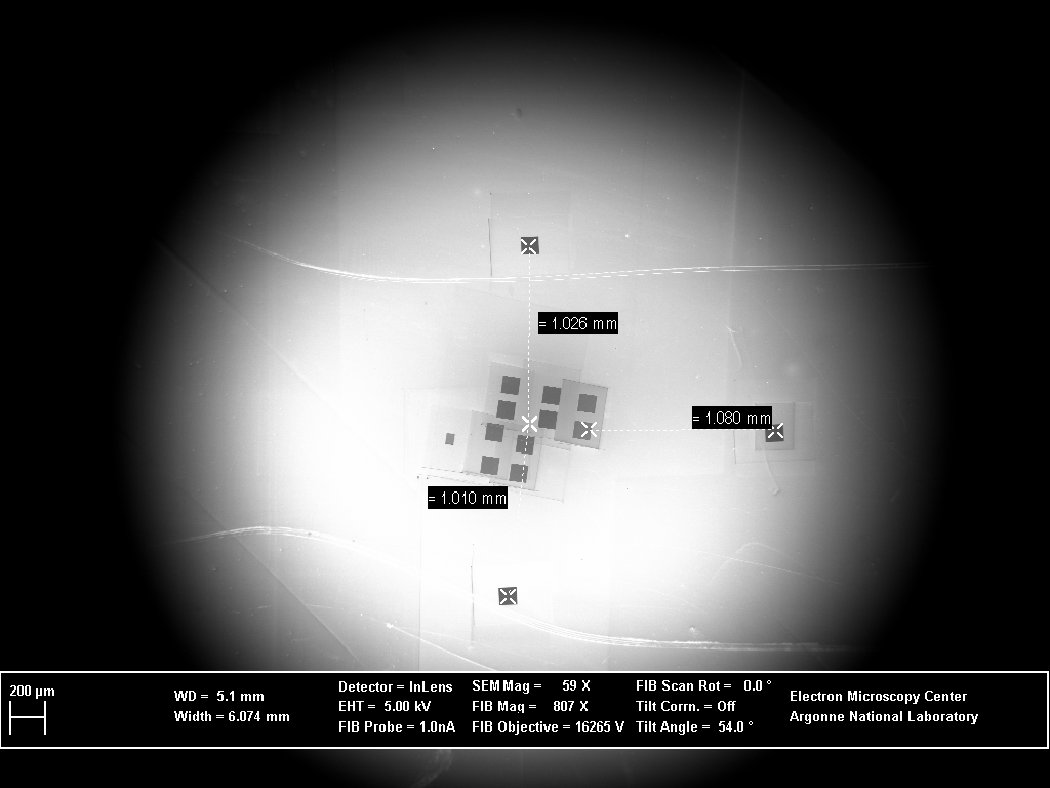
\includegraphics[width=2in]{FIB-medium}
      }
      ;
    }
    \begin{pgfonlayer}{below-main}
      \draw<3-> (low-top-left.center) -- (medium.north west);
      \draw<3-> (low-top-right.center) -- (medium.north east);
      \draw<3-> (low-bottom-left.center) -- (medium.south west);
      \draw<3-> (low-bottom-right.center) -- (medium.south east);
    \end{pgfonlayer}
    \begin{pgfonlayer}{above-main}
      \visible<5->{
        \node [
          inner sep=0,
          name=high,
          below right=1cm of medium.center,
          label=below:High Mag
        ] {
          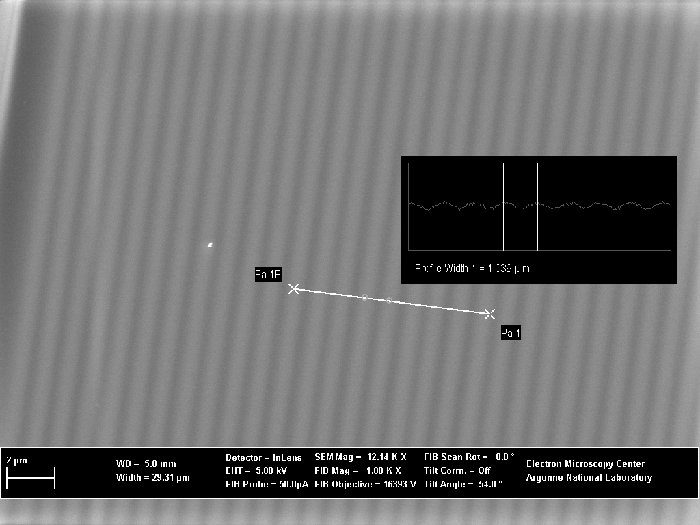
\includegraphics[width=2in]{FIB-high}
        };
      }
    \end{pgfonlayer}
    \node [name=feature, right=2.3mm of medium.center,inner sep=0.7mm,yshift=-0.5mm] {};
    \draw<4->
      (feature.north east)
      -- (feature.north west)
      -- (feature.south west)
      -- (feature.south east)
      -- cycle
    ;
    \draw<5-> (feature.north east) -- (high.north east);
    \draw<5-> (feature.north west) -- (high.north west);
    \draw<5-> (feature.south east) -- (high.south east);
    \draw<5-> (feature.south west) -- (high.south west);
  \end{tikzpicture}
\end{frame}

\begin{frame}{Sinusoidal Nanopatterned Photocathode: Results}
  \begin{center}
    \begin{tikzpicture}
      \node {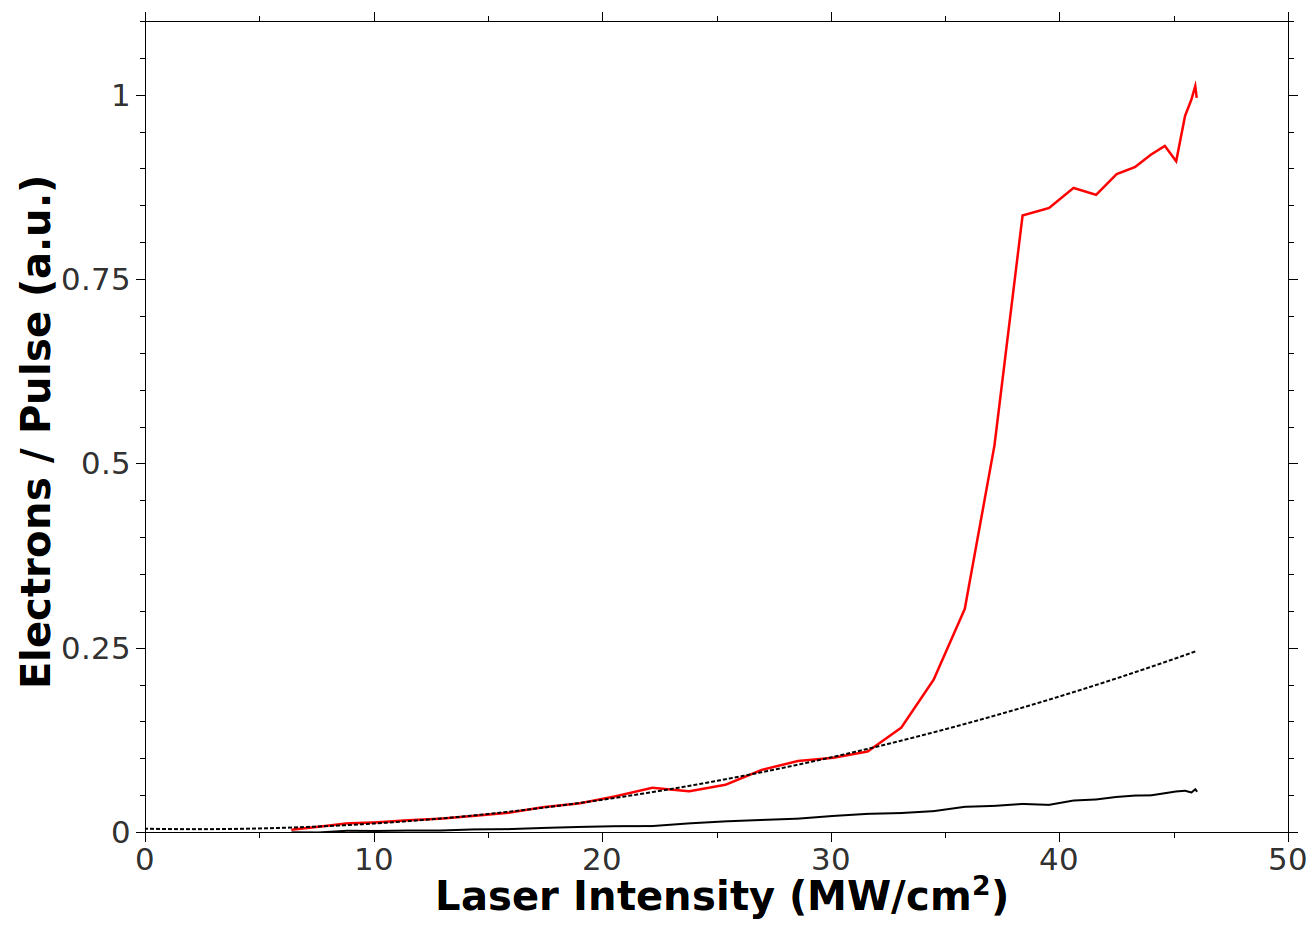
\includegraphics{Graph1}};
      \node<2> at (-1.8,1.8) [draw] {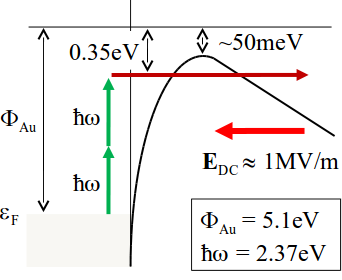
\includegraphics[width=1.2in]{PE_diag_0}};
      \node<3> at (-1.8,1.8) [draw] {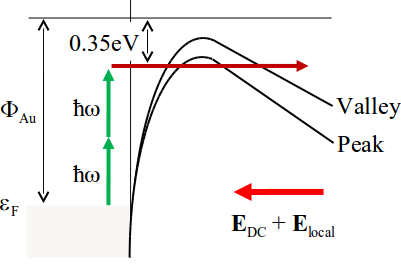
\includegraphics[width=1.2in]{PE_diag_1}};
      \node<4> at (-1.8,1.8) [draw] {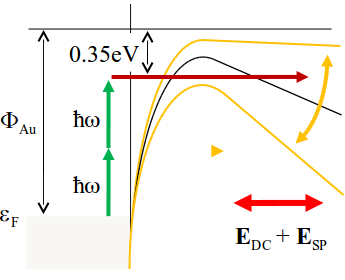
\includegraphics[width=1.2in]{PE_diag_2}};
      
      \node<1,3-4> at (2.1,2.8) [red,align=right] {Plasmon Enhanced\\Photoemission};
      \node<1> at (3.5,-0.7) {Fit $I^2$};
      
      \node<1-2> at (-1,-1.5) (TwoPhoton Label) [align=left] {Two Photon\\Photoemission};
      \draw<1-2> [thick,-latex]
        (TwoPhoton Label)
        to [out=0,in=110] (2.7,-2.2)
      ;
      
      \node<2> 
        at (3,1.7) 
        [label={below:Isotropic $\Delta p_{\scriptscriptstyle T}$}] 
        {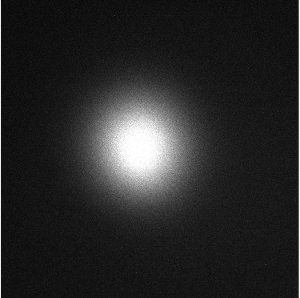
\includegraphics[width=1in]{final-fourier-2photon-036}}
      ;
      
      \node<3> 
        (fourier image)
        at (-2,-1) 
        [
          shape=rectangle callout, callout relative pointer={(0.9,-0.5)}, 
          draw, fill=white
        ] 
        {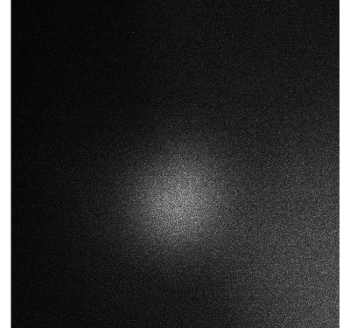
\includegraphics[width=1in]{final-fourier-022}}
      ;
      \node<3> [right=0.2 of fourier image] {Isotropic $\Delta p_{\scriptscriptstyle T}$};
      
      \node<4>
        at (-1.5,-1)
        [
          shape=rectangle callout, callout relative pointer={(1,-0.2)}, 
          draw, fill=white, align=left
        ] 
        {Onset of barrier suppression\\$\Rightarrow E_{SP} \approx$ 40MV/m}
      ;
      
      \node<5-> 
        at (-1.8,-1.4)
        [
          shape=rectangle callout, callout relative pointer={(1.9,-0.45)}, 
          draw, fill=white, align=left
        ] 
        {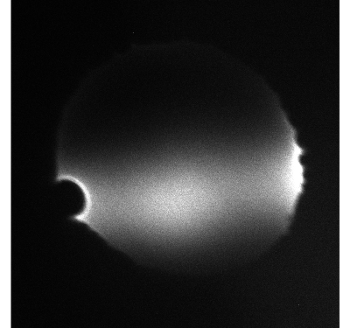
\includegraphics[width=0.7in]{final-fourier-026}}
      ;
      \node<5-> 
        at (0.5,0)
        [
          shape=rectangle callout, callout relative pointer={(0.7,-0.4)}, 
          draw, fill=white, align=left
        ] 
        {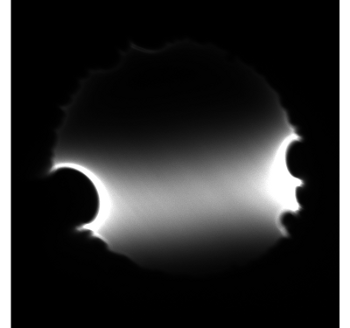
\includegraphics[width=0.7in]{final-fourier-030}}
      ;
      \node<5-> 
        at (1.2,2.2)
        [
          shape=rectangle callout, callout relative pointer={(1,0)}, 
          draw, fill=white, align=left
        ] 
        {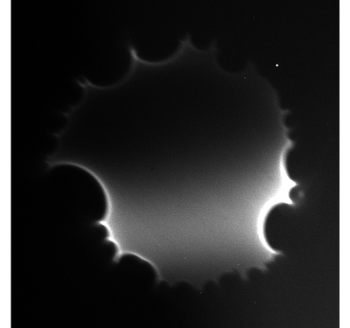
\includegraphics[width=0.7in]{final-fourier-038}}
      ;
      \node<5->
        at (-2,1.8)
        {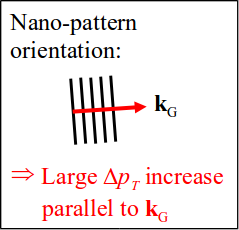
\includegraphics[width=1in]{PE_diag_3}}
      ;
    \end{tikzpicture}
  \end{center}
\end{frame}

\begin{frame}{Understanding Observed $\Delta p_{\scriptscriptstyle T}$ Increase}
  Is the 1D broadening due to the plasmon or the surface?
  \begin{center}
    \begin{tikzpicture}
  \draw [thick,->,green] 
    (0,0) -- ++(3,0) 
      node [pos=0.5,below,black,align=center] {$k_L \sin \theta$\\$\theta \approx 39^{\circ}$}
  ;
  \draw [thick,->,red]
    (3,0) -- ++(2,0)
      node [pos=0.5,below,black] {$k_G$}
  ;
  \draw [thick,->,blue]
    (0,0.2) -- ++(5,0)
      node [pos=0.5,black,above] {$k_{SP}$}
  ;
  \node at (7,0) {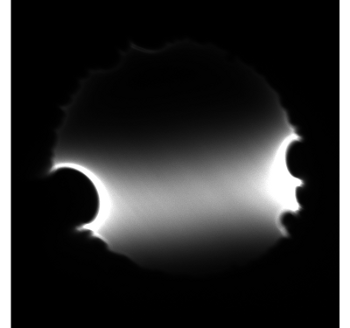
\includegraphics{final-fourier-030.png}};
  \draw [very thick,red] (6,-0.4) -- ++(9:2.2);

  \draw [thick,->,green] 
    (0,-3.5) -- ++(3,0) 
      node [pos=0.5,below,black,align=center] {$k_L \sin \theta$\\$\theta \approx 47^{\circ}$}
  ;
  \draw [thick,dashed,green] 
    (3,-3.5) -- (4,-3.5)
      node [above,black,pos=0.8] {$45^{\circ}$}
  ;
  \draw [thick,->,red]
    (3,-3.5) -- ++(1.4,1.4)
      node [pos=0.4,left,black] {$k_G$}
      coordinate [pos=1] (end)
  ;
  \draw [thick,->,blue]
    (0,-3.5) -- (end)
      node [pos=0.5,black,above] {$k_{SP}$}
  ;
  \node at (7,-3) {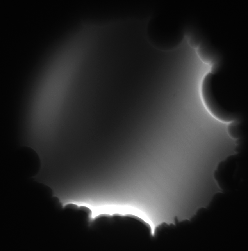
\includegraphics{rotated.png}};
  \draw [very thick,green,dashed] 
    (6,-2.7) -- ++(9:2.2)
      node [pos=0.7,below, white] {$45^{\circ}$}
      coordinate [pos=1] (rotate end)
  ;
  \draw [very thick,red]
    (rotate end) -- ++(234:2.2)
  ;
\end{tikzpicture}

  \end{center}
\end{frame}

\begin{frame}{Trenched Nanopatterned Photocathode}
  \begin{columns}
    \begin{column}{0.54\linewidth}
      Grooved Photocathode
      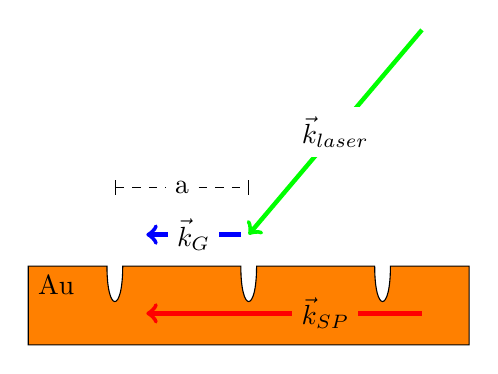
\begin{tikzpicture}
        \draw 
          [fill=orange]
          (0,0)
            node [below right] {Au}
          -- (1,0)
            .. controls (1,-0.6) and (1.2,-0.6)
          .. (1.2,0)
          -- (2.7,0)
            .. controls (2.7,-0.6) and (2.9,-0.6)
          .. (2.9,0)
          -- (4.4,0)
            .. controls (4.4,-0.6) and (4.6,-0.6)
          .. (4.6,0)
          -- (5.6,0)
          -- (5.6,-1)
          -- (0,-1)
          -- cycle
        ;  
        \draw [|-|,dashed]
          (1.1,1)
          -- (2.8,1)
            node [pos=0.5,fill=white] {a}
        ;
    
        \draw [ultra thick,red,->]
          (5,-0.6)
          -- (1.5,-0.6)
            node [pos=0.35,black,fill=orange] {$\vec{k}_{SP}$}
        ;
        \draw [ultra thick,green,->]
          (5,3)
          -- (2.8,0.4)
            node [pos=0.5,black,fill=white] {$\vec{k}_{laser}$}
        ;
        \draw [ultra thick, blue, ->]
          (2.7,0.4)
          -- (1.5,0.4)
            node [pos=0.5,black,fill=white] {$\vec{k}_{G}$}
        ;
      \end{tikzpicture}
    \end{column}
    \begin{column}{0.44\linewidth}
      \begin{align*}
        k_{SP} =& k_{laser}^{\parallel} + m \cdot k_{G}\\
        \sin(\theta) =& \sqrt{ \frac{\varepsilon}{1+\varepsilon} } - \frac{ m \lambda }{a}
      \end{align*}
      \begin{block}<2->{}
        \begin{itemize}
          \item Retains periodic structure
          \item Reduced $\nabla_{\perp} E_{SP}$
          \item Additional Fourier components
          \item Easier to FIB mill
        \end{itemize}
      \end{block}
    \end{column}
  \end{columns}
\end{frame}

\begin{frame}{Trenched Nanopatterned Photocathode: Results}
  \begin{columns}
    \begin{column}{0.49\linewidth}
      \begin{figure}
        \centering
        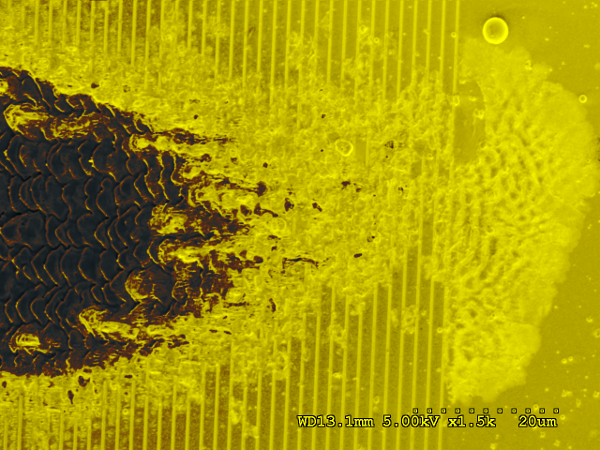
\includegraphics{trench_damage_false_color.png}
      \end{figure}
      \begin{itemize}
        \item Heat damage on grating
        \item Plasmon excitation?
      \end{itemize}
    \end{column}
    \begin{column}{0.49\linewidth}
      \begin{figure}
        \centering
        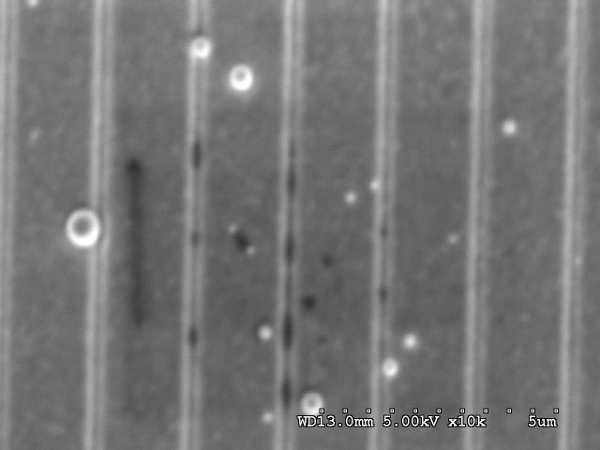
\includegraphics{trench_incomplete_filling.png}
      \end{figure}
      \begin{itemize}
        \item Incomplete filling of trenches
        \item Increases plasmon threshold 
        \item[$\Rightarrow$] laser damage 
      \end{itemize}
    \end{column}
  \end{columns}
  \vfill
  \begin{center}
    \alert{No evidence of plasmon-assisted photoemission!}
  \end{center}
\end{frame}

\begin{frame}
  \begin{columns}
    \begin{column}{0.45\linewidth}
      \begin{figure}
        \centering
        \begin{tikzpicture}
  % grid
  %\draw (-3,-2) grid (3,5);

  % axes
  \draw [-latex, thick] (-2.5,0) -- (2.5,0) node [below] {$k$};
  \draw [-latex, thick] (0,-1.5) -- (0,4) node [left] {$E$};

  % bands
  %\draw (-1,-0.5) .. controls (-0.25,0.25) .. (0,0);
  %\draw (-1,-1) .. controls (-0.5,0) and (0.5,0) .. (1,-1);
  \coordinate (so gamma) at (0,-0.5);
  \draw<3-> (so gamma) arc [start angle=90, end angle=30,  radius=1];
  \draw<3-> (so gamma) arc [start angle=90, end angle=150, radius=1]
    node [below] {SO};

  \coordinate (origin) at (0,0);
  \draw (origin) arc [start angle=90, end angle=50,  radius=2];
  \draw (origin) arc [start angle=90, end angle=130, radius=2]
    node [left] {HH};

  \draw (origin) arc [start angle=90, end angle=50,  x radius=1.5, y radius=4];
  \draw (origin) arc [start angle=90, end angle=130, x radius=1.5, y radius=4]
    node [left] {LH};

  \coordinate (cb gamma) at (0,0.5);
  \draw (cb gamma) arc [start angle=-90, end angle=-50,  x radius=1, y radius=4];
  \draw (cb gamma) arc [start angle=-90, end angle=-130, x radius=1, y radius=4]
    node [above] {CB};
  \node [left] at ($(cb gamma)!0.5!(origin)$) {$E_g$};

  \coordinate (gamma 8) at (0,2);
  \draw<2-> (gamma 8) arc [start angle=-90, end angle=-30,  radius=1.5];
  \draw<2-> (gamma 8) arc [start angle=-90, end angle=-150, radius=1.5]
    node [above] {$\Gamma_{8}$};

  \coordinate (gamma 7) at (0,1.95);
  \draw<7-> (gamma 7) arc [start angle=90,  end angle=30,   radius=1.5]
    node [below right] {$\Gamma_{7}$};
  \draw<7-> (gamma 7) arc [start angle=-90, end angle=-150, radius=1.5];
  \draw<7-> [green,->] (gamma 7) ++(0,0.15) arc [start angle=90,  end angle=30,   radius=1.5]
    node [right] {$\tau_{{\scriptscriptstyle decay}}$};

  % defined energies
  \coordinate (energies) at (-1.5,0);
  \draw<4-> [thick] ($(gamma 8) + (-2,0)$) -- ++(4,0);
  \draw<4-> [<->] (energies) -- (energies |- gamma 8)
    node [pos=0.5,left] {$E_{g}^{\prime}$};

  \coordinate (vacuum level) at ($(gamma 8) + (0,0.6)$);
  \draw [thick,red] ($(vacuum level) + (-2,0)$) -- ++(4,0)
    node [right,align=left,font=\tiny] {Vacuum\\Level};
  \draw<4-> [<->] (energies |- gamma 8) -- (energies |- vacuum level)
    node [pos=0.5,left] {$\phi$};

  % photon excitation
  \draw<1> [-latex, blue, very thick] (0.05,0) -- ++(0,2.54)
    node [right,pos=0.7] {$\hbar \omega$};
  \draw<3-> [-latex, blue, very thick] (0.1,-0.52) -- ++(0,2.54);
  \draw<2-> [-latex, blue, very thick] (0.63,-0.38) -- ++(0,2.54);
  \draw<2-> [-latex, blue, very thick] (0.9,-0.23) -- ++(0,2.54)
    node [right,pos=0.3] {$\hbar \omega$};

\end{tikzpicture}

      \end{figure}
    \end{column}
    \begin{column}{0.53\linewidth}
      \begin{tabular}{|c|c|c|}
        \hline
          & GaSb & InSb \\ \hline
        \rowvisible{4-}{$E_{g}^{\prime}$}{3.77eV}{3.59eV} \\ \hline
        \rowvisible{4-}{$\phi$}{0.99eV}{1.18eV} \\ \hline
        \rowvisible{5-}{Excess $E$}{$\sim$0.35eV}{$\sim$0.41eV} \\
        \rowvisible{5-}{$\Rightarrow$ initial $T_e$}{4200K}{4900K} \\ \hline
        \rowvisible{8-}{$m^{*}(\Gamma_8)$}{$0.3 m_0$}{$0.5 m_0$} \\ \hline
      \end{tabular}
      \vspace{3mm}
      \visible<6->{
        $\exp(-\phi / k_{{\scriptscriptstyle B}} T_e) \approx 0.6$
        \begin{itemize}
          \item thermionic photoemission!
        \end{itemize}
      }
      \visible<7->{
        Cooling rates of $\sim$1600 K/ps from
        \begin{itemize}
          \item LO phonons 
          \item fast decay via $\Gamma_7$
        \end{itemize}
      }
    \end{column}
  \end{columns}
\end{frame}
